
All code was implemented in the Julia language due to the availability of \textit{packages} for subproblems of this work. In the next section, several components of the solution to the problem of optimization of impulsive maneuvers are detailed, and the following section assembles all components into the full optimization algorithm.

TODO multiple shooting is dynamics agnostic

\section{Components}

The optimization of impulsive maneuvers relies on the representation and manipulation of several concepts in a programmatic fashion. In particular there is a need for a numerical way of propagating orbits, a representation for sequences of impulses and coasting arcs, an implicit formulation for maneuvers amenable to optimization, and a way of calculating primer vector trajectories on multi-impulse maneuvers. Each of those components will be explored in the following sections.

\subsection{Orbit Propagation}\label{sec:orbit_propagation}

The implementation of an orbit propagator concerns itself with the implementation of the function \(p_o(\mathbf{x}, t)\) introduced in Equation~\eqref{eq:orbit_propagator}. Two different cases are to be considered: ``explicit'' propagation, where numerical inputs are available and a numerical output is desired; and ``implicit'' propagation, where the propagation step is a part of a larger solver.

Brazil's National Institute of Space Research (INPE) developed a package for orbit propagation and analysis with several models (Kepler, J2 semi-analytical secular and short term, among others) called \texttt{SatelliteToolbox}~\cite{satellitetoolbox}. It provides quite convient functions for converting between the Cartesian state vector \(\begin{bmatrix}
    \mathbf{r}^T & \mathbf{v}^T
\end{bmatrix}^T\) and the Keplerian elements, as well as functions for the propagation of orbits by some specified amount of time \(t_p\). Its algorithms were chosen with precision around edge cases in mind~\cite{rv_to_kepler}, making it numerically precise but unsuitable for nonlinear solvers, which expect differentiable functions everywhere. The functions in this package are also limited to elliptic orbits, which are not guaranteed to be found during iteration inside a numerical solver like Ipopt.

Therefore, this is an auxiliary package used for verification, initial guess generation, and direct numerical propagation whenever required. When propagation is required in the statement of a nonlinear optimization problem, another method for orbit propagation is required. Despite being useful for explicit propagation, Keplerian elements are unsuited for optimization (at least with the chosen solver, see Section~\ref{sssec:solver}). This can be seen from the equation relating the true anomaly \(\theta\) and the eccentric anomaly \(E\), Equation~\eqref{eq:true_exc_anom}, discussed in Table~\ref{tab:kep_ecc_true}. In summary, the anomaly equations require special treatment close to the apogee to avoid infinities or discontinuities.

\begin{table}[htbp]
    \centering
    \begin{tabular}{cccc} \toprule
        Form & LHS value at apogee & RHS value at apogee & Comment  \\ \midrule
        \(\tan{\frac{\theta}{2}} = \sqrt{\frac{1+e}{1-e}} \tan{\frac{E}{2}}\) & \(+\infty\) & \(+\infty\) & \parbox{2.5cm}{Value unsuitable for computation} \\
        \(\theta = 2\arctan{\sqrt{\frac{1+e}{1-e}} \tan{\frac{E}{2}}}\) & \(\pi\) & \(\pm\pi\) & \parbox{2.5cm}{Not continuous \(\therefore\) not differentiable} \\ \bottomrule
    \end{tabular}
    \caption{Problems with the Keplerian elements formulation exemplified with the relationship between eccentric and true anomalies}
    \label{tab:kep_ecc_true}
\end{table}

Therefore, the dynamics in Cartesian coordinates were chosen for implicit propagation, due to the differentiability of this model in the usual range of orbital variables. Many methods for integrating dynamical systems for optimal control exist, such as collocation, pseudospectral methods, direct shooting, and multiple shooting~\cite{numerical_recipes}. Multiple shooting was chosen since it leads to a numerically stable problem and is standard in optimal control. An eighth-order Runge-Kutta (RK8) method~\cite{rk8} was used for discretizing the dynamical equations. Let  \(\mathbf{x}_{\text{next}} = f_{RK}(\mathbf{x}_{\text{prev}}, \Delta t)\) be the RK8 integration function from Cartesian state \(\x_{\text{prev}}\) to Cartesian state \(\mathbf{x}_{\text{next}}\) over a time step \(\Delta t\).

The multiple shooting implicit orbit propagation uses \(N\) discretization points for a coasting arc of duration \(d_c\), which are parameterized with Cartesian state vector variables \(\x^j \in \R^6, j=1,\dots,N\) subject to 
\begin{equation}
    \mathbf{x}^{j+1} = f_{RK}(\frac{d_c}{N - 1}, \mathbf{x}^j), j = 1, \dots, N.
\end{equation}

To complete the implicit description, \(\dim \mathbf{x} = 6\) boundary conditions are needed. These may be an initial condition, a final condition, or an impulsive boundary condition between two arcs.

%this part is messy
% Let \(\mathbf{x}_{\text{next}} = f_{RK}(\mathbf{x}_{\text{prev}}, \Delta t)\) be the dynamics function discretized through the eighth order Runge Kutta method. Then a number \(N\) of discretization points is chosen and \(N\) state vector variables \(\mathbf{x}^j, j=1,\dots,N\) are created belonging to an array \(\chi \in \mathbb{R}^{6 \times (N)}\). They are subject to the constraints
% \begin{equation}
%     \mathbf{x}^{j+1} = f_{RK}(\mathbf{x}^j, \frac{t_p}{N}), j = 1, \dots, N.
% \end{equation}
% This leaves \(\dim \mathbf{x} = 6\) degrees of freedom, which are to be specified with a boundary condition. This boundary condition can be an initial condition, a final condition or relation to another coasting segment through an impulse, as will be discussed in Section~\ref{sec:impulsive_statement}. Thus, this parameterization of orbital propagation is \textit{isoconstrained}.

\subsection{Maneuver Propagation}\label{sec:maneuver_propagation}

Impulsive maneuvers are characterized by a sequence of impulses and coasting arcs. A notation for maneuvers is introduced, where \texttt{C} represents a coasting arc, and \texttt{I} represents an impulse. Any alternating sequence \(\mathcal{S} \in \{\texttt{C}, \texttt{I}\}^{n_c + n_i}\), where \(n_c\) is the number of coasting arcs and \(n_i\) is the number of impulses, with 2 or more impulses makes a valid maneuver: \texttt{ICI}, \texttt{ICIC}, \texttt{CICICICIC}, etc. Maneuvers need at least 2 impulses to be able to take any initial state to any final state (see Section~\ref{sec:imp_prop_model}). Also, let \(\mathcal{I} = \{i \in 1,\dots,n_i+n_c | \mathcal{S}_i = \texttt{I}\}\) and \(\mathcal{C} = \{c \in 1,\dots,n_i+n_c | \mathcal{S}_c = \texttt{C}\}\) be the sets of impulse and coast indices respectively. Figure~\ref{fig:maneuver_propagation} illustrates the algorithm for propagating a maneuver: at impulses, a velocity discontinuity is applied; at coasting arcs, the orbit is propagated. This algorithm follows the specified sequence of maneuvers for given values of impulse magnitudes and directions, and coast durations. 

Implicit maneuver propagation is required for optimization. For this, coasts are parameterized according to the multiple shooting scheme of last section, and impulsive boundary conditions between arcs are added as constraints.  


\begin{figure}[htbp]
    \centering
    \begin{tikzpicture}
        \node (init) [startstop] {Initial state};
        \node (dots1) [process, right = of init] {\ldots};
        \node (imp) [process, below = of dots1] {\textbf{Impulse}
        
        Velocity discontinuity};
        \node (coast) [process, right = of imp] {\textbf{Coast}
        
        Orbit 
        
        propagation};
        \node (dots2) [process, below = of coast] {\ldots};
        \node (final) [startstop, right = of dots2] {Final state};

        \draw [arrow] (init) -- (dots1);
        \draw [arrow] (dots1) -- (imp);
        \draw [arrow] (imp) -- (coast);
        \draw [arrow] (coast) -- (dots2);
        \draw [arrow] (dots2) -- (final);

    \end{tikzpicture}
    \caption{Maneuver propagation scheme.}
    \label{fig:maneuver_propagation}
\end{figure}

%talk about random start, stopping early
%talk about primer vector algorithm
%talk about repropagation

\subsection{Maneuver multiple shooting problem statement}

The full maneuver optimization problem, in its multiple shooting formulation, shall be stated in this section. The input parameters are:
\begin{enumerate}
    \item \(\mathbf{r}_1\), \(\mathbf{v}_1\): initial orbital position and velocity;
    \item \(\mathbf{r}_2\), \(\mathbf{v}_2\): final orbital position and velocity;
    \item \(t_f\): transfer time;
    \item \(N\): number of integration steps per coasting arc.
    \item \(\mathcal{S} \in \{\texttt{C}, \texttt{I}\}^{n_c + n_i}\): the desired sequence of coasts and impulses.
\end{enumerate}

The problem's definition and variable set dynamically depends on the input sequence. The \(i\)-th impulse is described by the variables\footnote{The problem could have been parameterized with vector quantities for the changes in velocities, \(\Delta \vec{\mathbf{v}}\), but the objective function would then be stated \(\sum \sqrt{\Delta \vec{\mathbf{v}}^T \Delta \vec{\mathbf{v}}}\), which is not differentiable at \(\Delta \vec {\mathbf{v}} = 0\), which is inconvenient.}
\begin{enumerate}
    \item \(\Delta v_i \geq 0\): magnitude of the impulse;
    \item \(\hat{\uc}_i \in \R^3\): direction of the impulse.
\end{enumerate}

The \(c\)-th coasting arc is described by:
\begin{enumerate}
    \item \(d_c \geq 0\): total duration of the arc;
    \item \(\x^j_c \in \R^6, j=1,\dots,N\): tate vector variables for each coasting arc. 
\end{enumerate}

Some care needs to be taken about the first sequence element, an impulse or coast, since this changes the necessary constraints for the initial and final conditions. The full multiple shooting problem for the optimization of the impulsive maneuver is:

\begin{align}\label{eq:ms_problem}
    \begin{tabular}{cl}
     \(\min\)                              & \(\sum_{i \in \mathcal{I}} \Delta v_i\)\\
    \(\Delta v_i  \in \R_+, i \in \mathcal{I}\), &  \\
    \(\hat{\uc}_i \in \R^3, i \in \mathcal{I}\),     & \\
    \(d_c         \in \R_+, c \in \mathcal{C}\),     & \\
    \(\x^j_c      \in \R^6, j=1,\dots,N, c \in \mathcal{C}\) & \\
    \textbf{subject to:}        & \\
    Total time                  & \(\sum_{c \in \mathcal{C}} d_c = t_f\) \\
    Unit directions             & \(\hat{\uc}_i^T \hat{\uc}_i = 1, i \in \mathcal{I}\) \\
    Propagation of coasts       & \(\x^{j+1}_c = f_{RK}(\frac{d_c}{N-1}, \x^j_c)\), \\
                                & \(j=1,\dots,N-1, c \in \mathcal{C}\) \\
    Impulse boundary conditions & \(\x^1_{i+1} = \x^{N}_{i-1} + \begin{bmatrix}
        0_{3\times1} \\ \Delta v_i \hat{\mathbf{u}}_i
    \end{bmatrix}\), \\
                                & \(i \in \mathcal{I}, i \neq 1, n_i+n_c\) \\
    Initial condition           & \(\x_1^1 = \begin{bmatrix}
        \mathbf{r}_1 \\ \mathbf{v}_1
    \end{bmatrix}, 1 \in \mathcal{C}\) \\
                                & \(\x_2^1 = \begin{bmatrix}
                                    \mathbf{r}_1 \\ \mathbf{v}_1 + \Delta v_1 \hat{\mathbf{u}}_1
                                \end{bmatrix}, 1 \in \mathcal{I}\) \\
    Final condition             & \(x_c^N = \begin{bmatrix}
        \mathbf{r}_2 \\ \mathbf{v}_2
    \end{bmatrix}, c = n_i+n_c \in \mathcal{C}\) \\
                                & \(x_{i-1}^N + \begin{bmatrix}
                                    0_{3\times1} \\ \Delta v_i \hat{\mathbf{u}}_i
                                \end{bmatrix} = \begin{bmatrix}
                                    \mathbf{r}_2 \\ \mathbf{v}_2
                                \end{bmatrix}, i = n_i+n_c \in \mathcal{I}\)
    \end{tabular}
 \end{align}

% The solver should be initialized with a feasible, but not necessarily optimal solution, for better convergence (since Ipopt is a local solver, the choice of initial guesses is important). Values for \(\Delta t_1\) and \(\Delta t_2\) should be proposed based on physical reasoning. Then, the variables of the first and last coasting arcs are initialized with direct orbital propagation results (computed with the \texttt{SatelliteToolbox} package). The second coasting arc, between the impulses, is initialized with the solution to the Lambert problem between the final position of the first coasting arc and the initial position of the last coasting arc. Finally, the variables concerning the impulses' magnitudes and directions are initialized with the difference in velocity between consecutive arcs.

As discussed in Section~\ref{sssec:solver}, the solver should be initialized with an initial guess that is not far from being feasible. For multiple shooting schemes, this means satisfying the dynamical constraints, but possibly not the final condition constraint. Therefore, initial guesses can be generated by guessing impulse magnitudes and directions, coast durations and applying the maneuver propagation algorithm from Section~\ref{sec:maneuver_propagation}. dc, random start

\subsubsection{Nonlinear solver}\label{sssec:solver}

Nonlinear solvers are algorithms which iteratively approximate the solution to a system of nonlinear equations or a constrained optimization problem. Many algorithms, and many different algorithms exist. Optimizer algorithms may be classed as local or global, depending on whether they find a local (best in a region) or global (best in the domain) solution; stochastic, according to the presence or absence of random seeding; and the usage of function evaluations only, gradient evaluations, or even Hessian evaluations~\cite{numerical_recipes}. All local methods require an initial guess as input.

Of interest to this work are deterministic local gradient-based algorithms. They are well suited to nonlinear (but continuous and differentiable) problems with continuous variables subject to nonlinear constraints. By exploiting the gradient, faster algorithms are available. The choice for a local, deterministic solver comes from the fact that these algorithms have much faster convergence than global stochastic algorithms such as simulated annealing. To make up for the loss of global optimality, good initial guesses must be supplied.

Julia offers a multitude of nonlinear solvers, each with different scope, interface, and algorithms. This work has chosen to use \texttt{JuMP}~\cite{jump}, a package which offers a modelling language for optimization problems that is quite close to mathematical notation. The package's \textit{tech stack} can be seen in Figure~\ref{fig:tech_stack}. Internally, \texttt{JuMP} relies on an intermediary package, \texttt{MathOptInterface}, which standardizes solver interfaces. This in turn allows for the usage of \texttt{Ipopt\_jll}, an unofficial wrapper for the Ipopt solver. Ipopt is an open-source nonlinear solver widely recognized for its speed and precision, outperforming many competitors and being quite flexible. It is especially well suited to problems with many variables (up to thousands) with sparse constraints (that is, constraints that depend only on small subsets of variables). It is capable of handling equality and inequality constraints.

This solver allows for the specification of lower and upper bounds of variables separately to the specification of inequality constraints. Variable bounds are guaranteed to be respected at all iterations; inequality constraints are only guaranteed to be satisfied at the converged solution, if the problem is feasible. This distinction is important because some constraints define the domain of problem and should never be violated; other constraints are problem-based and therefore can be violated during the iteration process.

Finally, Ipopt is built with sparsity in mind. Complex calculations should be broken into simpler constraints, each depending on less variables. This may even increase the number of variables but Ipopt's performance profits from this structure.

\begin{figure}[htbp]
    \centering
        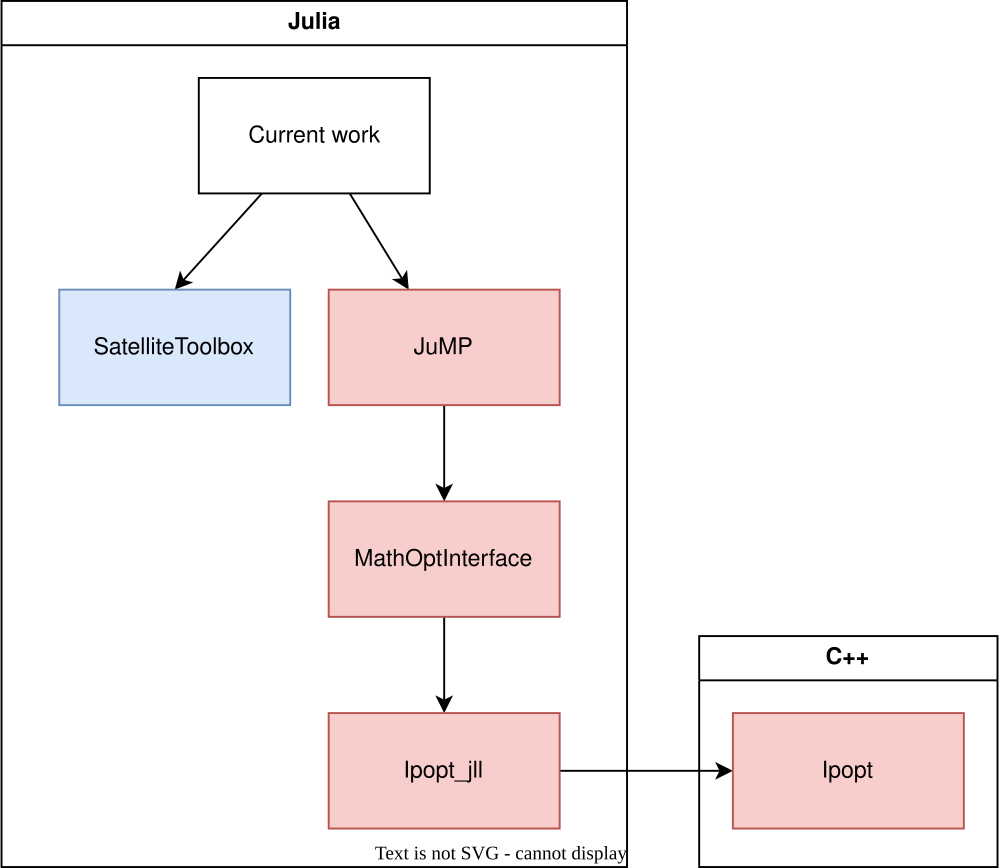
\includegraphics[width=\textwidth]{img/techstack.png}
    \caption{Relationship of code components.}
    \label{fig:tech_stack}
\end{figure}
%flowchart

\subsubsection{Variable normalization}

\subsection{Primer vector algorithm}

\begin{tikzpicture}
    \node (linearTPBVP) [process] {Solve linear TPBVP between pair of impulses};
    \node (firstcoast) [process, right = of linearTPBVP] {Backpropagate PV if \texttt{C...}};
    \node (lastcoast) [process, below = of firstcoast] {Propagate PV if \texttt{...C}};
    \node (diag) [decision, right = of firstcoast, text width=2cm] {Necessary conditions};
    \node (opt) [startstop, below = of diag] {Local optimum};
    \node (cont) [startstop, right = of diag] {More impulses};

    \draw [arrow] (linearTPBVP) to [out=45, in=90, looseness=3] (linearTPBVP);
    \draw [arrow] (linearTPBVP) -- (firstcoast);
    \draw [arrow] (firstcoast) -- (diag);
    \draw [arrow] (linearTPBVP) -- (lastcoast);
    \draw [arrow] (lastcoast) -- (diag);
    \draw [arrow] (diag) -- (opt);
    \draw [arrow] (diag) -- (cont);
\end{tikzpicture}

% \section{Lambert problem implementation}

% The formulations stated in the previous chapter make for one-dimensional nonlinear programs, which leads to high performance. However, they do not handle the singularity case of \(r_1 \parallel r_2\), which is of particular importance to orbital maneuvers as they often happen at periapsis and apoapsis. Sukhanov's formulation actually gives expressions for the initial radial and normal velocity when the input positions are collinear; the plane of the orbit should then be adequately chosen afterwards~\cite{sukhanov}. However, this was found to be very numerically sensitive and another algorithm was used in the rest of this work. An implicit orbit propagation algorithm, as described in Section~\ref{sec:orbit_propagation} is setup with boundary conditions

% \begin{align}
%     \mathbf{r}_{(j=1)}   &= \mathbf{r}_1 \\
%     \mathbf{r}_{(j=N+1)} &= \mathbf{r}_2
% \end{align}
% which account for the 6 boundary conditions needed. In order to help convergence in the collinear case (and neighboring cases), two inequality constraints may be added:
% \begin{align}
%     \mathbf{r}_j^T \mathbf{r}_j &\geq R_{\text{Earth}}^2 \\
%     \mathbf{r}_j \times \mathbf{v}_j &\geq 0
% \end{align}
% where the second constraint must be inverted if the desired orbit is retrograde. 

% The propagation variables are initialized with the initial position and velocity.


\section{Primer vector meta-algorithm}\label{sec:impulsive_statement}



\begin{tikzpicture}
    \node (2r) [startstop] {\texttt{ICI} Case};
    \node (2f) [process, right=of 2r] {\texttt{CICIC} Case};
    \node (pv) [decision, right=of 2f] {PV trajectory};
    \node (more_imp) [process, right=of pv] {Add one impulse \texttt{C} \(\rightarrow\) \texttt{CIC}};
    \node (end) [startstop, below=of pv] {Local Optimum};

    \draw [arrow] (2r) -- (2f);
    \draw [arrow] (2f) -- (pv);
    \draw [arrow] (pv) -- (more_imp);
    \draw [arrow] (pv) -- (end);
    \draw [arrow] (more_imp.north) |- (pv.north);
\end{tikzpicture}